\documentclass[a4paper, 11pt]{scrartcl}
\usepackage{fullpage}
\usepackage{graphicx}
\usepackage{appendix}
\usepackage{booktabs}

% hyperref and nameref so that we can have sane internal refs
% hyperref also helps with pdf index creation
\usepackage{hyperref}
\usepackage{nameref}

% Place all of the figures at the end of the document
\usepackage[figuresonly,nomarkers,nolists]{endfloat}
\renewcommand{\efloatseparator}{}

\newcommand{\sryear}{2015}

\hypersetup{pdftitle = {Student Robotics \sryear\ Rulebook},
            bookmarks = {true},
            bookmarksopen = {true},
            bookmarksopenlevel = {0},
            bookmarksnumbered = {true},
            hypertexnames = {false},
            colorlinks = {true},
            linkcolor = {blue},
            citecolor = {blue},
            urlcolor = {red},
}

\title {Student Robotics \sryear\\ Rulebook}
\author{Revision 4}
\date{\today}

\begin {document}
\maketitle

\noindent The following defines the rules and regulations of the Student Robotics \sryear {} competition.  The latest version of this document can be found at \url{https://www.studentrobotics.org/rules}.

\newcounter{rule}[section]
\newcommand{\rcn}{\stepcounter{rule}\arabic{section}.\arabic{rule}}
\renewcommand{\labelenumi}{\rcn}

\section {Game Rules}
\label{game-rules}

\begin{enumerate}
\item The game, called \textbf{Pirate Plunder}, will be played in the arena defined in section~\ref{sub:arena}.
      The objective of this game is to achieve as many points as possible by collecting tokens,
       placing them on pedestals, and moving tokens into the team's zone.

\item Before a match starts, the teams participating in that match will be given some time to set their robot up in the arena.
      During this time, they:
\begin{enumerate}
  \item Must place their robot in the zone that they are assigned.
        The robot must be placed such that it is entirely within this zone, with no parts overhanging its boundary.

  \item Must ensure their robot has four robot badges attached it.
        These will be provided by Student Robotics officials at the beginning of the set-up time.
        Section~\ref{sec:robot-badges} provides more information about these markers, as well as their dimensions and mounting requirements.
\end{enumerate}
      Once all robots have been arranged, 20 tokens will be placed in the arena centre.

\item A match lasts 180 seconds.

\item At the end of a match, each team's ``\textbf{game points}'' will be calculated.
      These are used to rank teams before competition league points are awarded.
      Game points will be awarded as follows:
\begin{itemize}
  \item \textbf{1 point} will be awarded for each token that the robot is carrying.
  \item For each token that is entirely within, and in contact with the floor of the team's zone, \textbf{2 points} will be awarded.
  \item \textbf{5 points} will be awarded for each token that is atop the team's pedestal.

\end{itemize}

\item A robot will be considered to be carrying a token if the token's weight is fully supported by the robot, and the token is not in contact with any part of the arena (walls, floor, etc.).
      The judge may ask a member of the robot's team -- or a member of Student Robotics staff -- to lift the robot to demonstrate which tokens are supported by the robot -- if the token moves with the robot, and does not fall off, then it is supported by the robot.

\item At the end of a game, league points will be awarded as follows.
      The team with the \emph{most} game points will be awarded 4 points towards the relevant competition league.
      The team with the second most will be awarded 3.
      The team with the third most will be awarded 2 points, and the team with the fewest game points will be awarded 1 point.
      Teams whose robot was not entered into the round, or who were disqualified from the round, will be awarded no points.

      Tied robots will be awarded the average of the points that their combined positions would be awarded.
      Thus, three robots tied for first place would receive 3 points each (since this is $(4+3+2)/3$).

\item The competition will be structured in two leagues: the \textbf{silver} league, and the \textbf{gold} league.
      Teams will take part in \textbf{6} placement matches each. The upper 5 teams will qualify for gold league, the lower 5 will qualify for silver league.
      Matches will then alternate between leagues, with each team taking part in \textbf{4} matches within that league.
      Finally, the top 4 teams from each league will compete in a final for that league.
      The exact match schedule is documented in Appendix~\ref{apx:matches}.

\item There will be a maximum of 4 robots in a match.
\item Robots will be started by teams leaning into the arena to press the start button on their robot\footnote{A wireless match-starting solution may be provided by Student Robotics} when instructed to do so.

\item There must be no team members in the arena during the 1 minute before a match is scheduled to start.
      Robots must be installed and oriented before this deadline.
      During this minute there must be no interaction with the robot.
      Teams that do not meet this rule will forfeit the match.

\item A match may be terminated prematurely if all teams participating in that match state to the judge that they are happy for the game to end.

\item A token will be considered to be on a pedestal if the token is fully supported by the pedestal, and no part of the token is in contact with a robot, or any other part of the arena.

\end{enumerate}

\newpage
\section {Regulations}
\label{sec:Regulations}

\begin{enumerate}

%% Behaviour

\item No remote control systems may be used.
\item This is a non-contact sport, but accidental bumps and scrapes are inevitable.
\item Robots must not intentionally damage anything -- including tokens, pedestals, the arena or other robots.
\item Student Robotics reserves the right to examine your robot software and hardware at any time.
\item Assistance from Student Robotics Engineers is provided without any guarantees.
\item All kit deployed by Student Robotics remains the property of Student Robotics.
      All kit \textbf{must} be returned to Student Robotics after the competition.

\item The Judge's decision is final.

%% Physical

\item Robots must pass an inspection by a Student Robotics Inspector before competing in a match.
      This inspector will check that the robot complies with the rules and regulations of this game.
      \textbf{Robots that have not passed inspection may not be permitted to compete}.

\item At the beginning of each match, robots must fit within a cube with $500mm$ internal sides.

\item The power board, including its power switch, must be easily accessible at all times -- including throughout the game.
      This is for everyone's safety, especially your robot's.

\item All custom electronics that require a connection to the battery must instead be connected to the motor rail.
      There are extra connectors on the power board for this purpose.

\item All wires connected to the robot's ground (0V line) must be black.
      Black wires \emph{must not} be used for anything else.
      It is \emph{strongly recommended} that all wiring is neat and easily removable, as this will reduce the time required to debug problems on robots
       (teams may be asked to tidy their wiring before a Student Robotics Engineer will approach any issues with their robot).

\item All electronics must be securely fixed to the robot, and should also be easily removable.

\item It must not be possible to injure oneself on the robot.
      This will be tested using a Frankfurter sausage to simulate a finger.
      For example, high-speed rotating parts that could cause injury must be suitably shielded.

\item Robots must feature four mountings for robot badges.
      These mountings must comply with the specification in section~\ref{sec:robot-badges}.

\item The lithium-ion polymer batteries provided in the kit must be shielded from mechanical and thermal harm.
      This includes mechanical protection from accidental impact with other robots.
      Teams found to be in violation of this rule will have their batteries confiscated until they have demonstrably rectified the identified issues.

\item If teams wish to use batteries other than the lithium-ion polymer batteries provided,
       then they must seek approval from Student Robotics through the Student Robotics forums first.
      Additionally, if teams wish to add systems powered by separate batteries then they must seek approval through the same channel first.

      In general, teams are encouraged to power everything off the SR-supplied battery through the power board.
      All electromechanical components \textbf{must} be powered through the motor rail provided by the power board.

\item Robots may not include radio transmitters or receivers.
      In exceptional circumstances, teams may request an exemption from this rule.

\end{enumerate}

\newpage
\section{Specifications}
\label{sec:Specifications}

\newcounter{rulei}[subsection]
\newcommand{\rcnii}{\stepcounter{rulei}\arabic{section}.\arabic{subsection}.\arabic{rulei}}
\renewcommand{\labelenumi}{\rcnii}

\subsection{Markers}
\label{sub:markers}
The arena, tokens, buckets, and robots involved in the game are labelled with \textit{libkoki} markers.
Each marker pattern encodes a number.
Each marker number is associated with a particular feature within the arena, and also has an associated size.
The marker numbers and sizes are as follows:

\begin{center}
  \begin{tabular}{lcc}
    \toprule
    \textbf{Item} & \textbf{Marker Numbers} & \textbf{Marker Size (mm)} \\
    \midrule
    Arena boundary & 0 -- 27 & 250 \\
    Robots & 28 -- 31 & 100 \\
    Pedestal & 32 -- 35 & 200 \\
    Tokens & 36 -- 75 & 100 \\
    \bottomrule
  \end{tabular}
\end{center}

Two sets of marker codes will be used: one for development purpose, and one for the competition itself.
The competition set is only to be used inside the Student Robotics arena at the Student Robotics competition.
This is so that people carrying markers past the arena do not confuse robots.
The competition codes are 100 above the development codes.
When run in competition mode (specifiable through the robot's GUI), the software provided by Student Robotics will subtract 100 from the detected marker codes, as well as ignore the development codes.

The markers can be printed on a black-and-white printer.
Marker designs can be downloaded from the documentation section of the Student Robotics website.

Unless specified otherwise, all markers described in this document are oriented vertically such that the principle corner of the marker (which is indicated by a dark grey dot in the black marker border) is on the higher edge.

\subsection{Robot Badges}
\label{sec:robot-badges}

\begin{figure}
  \centering
  \includegraphics{./images/robot-marker.pdf}
  \caption{An example robot badge.
 The blue areas shown are the human-compatible areas.}
  \label{fig:example-badge}
\end{figure}

\begin{enumerate}
\item A ``robot badge'' is a removable identifier that will be attached to a robot throughout a match.
      It features the robot's assigned marker for the match, as well as human-compatible areas to allow spectators to easily associate a robot with its zone.
      An example of one of these badges is shown in figure~\ref{fig:example-badge}.
      The markings in the human-compatible areas are intentionally not specified.

\item A robot must feature four of the badge mounts shown in figure~\ref{fig:badge-mounting}.
      These mounts must permit a flat $200 \times 100mm$ panel to be attached to them.
      The three areas of each mount must feature the illustrated areas of hook-type Velcro to allow this panel to be fitted.

\item The four badge mounts must be on the exterior of the robot, parallel with the vertical plane, and should be perpendicular to each other about the vertical axis
      The orientation of the badge mounts is unimportant, but teams are encouraged to position them horizontally as shown in figure~\ref{fig:example-badge}.

  \begin{figure}
    \centering
    \includegraphics{./images/badge-mounting.pdf}
    \caption{The dimensions of the required robot badge mountings.
 The shaded areas are hook-type Velcro.
 All dimensions are in millimetres.}
    \label{fig:badge-mounting}
  \end{figure}
\end{enumerate}

\subsection{Arena}
\label{sub:arena}
\begin{enumerate}
\item The match arena floor, overall, is an $8m \times 8m$ square, as shown in figure~\ref{fig:arena-dim}.
      The tolerance of these two dimensions is $\pm0.25m$.

\begin{figure}
  \centering
  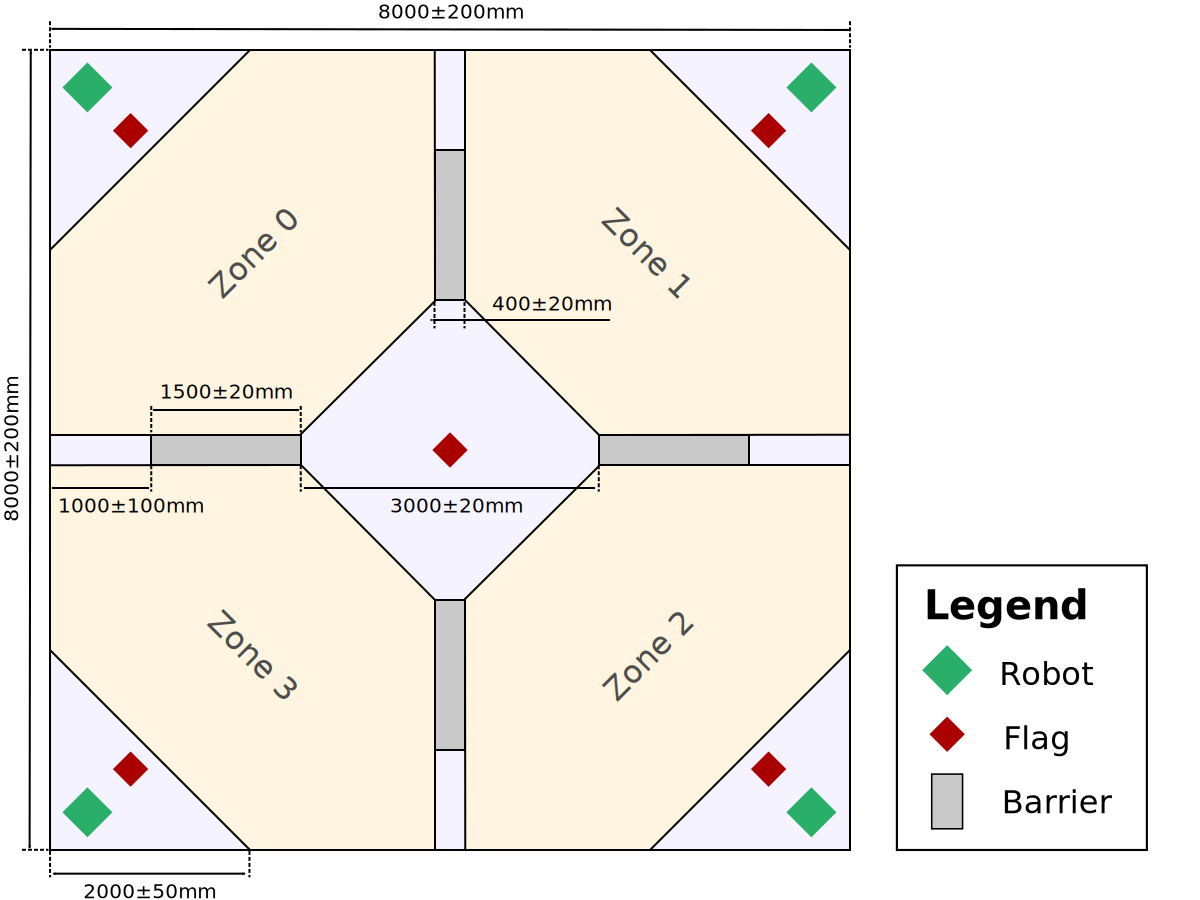
\includegraphics[width=0.8\textwidth]{./images/arena.pdf}
  \caption{\label{fig:arena-dim}A bird's-eye view of the arena.}
\end{figure}

\item \textbf{TODO}: Specify the arena centre area.

\item The floor of the arena is carpeted.
      The carpet tiles used in the arena are from B\&Q, with EAN 5014957151543.

\item The arena walls are $600\pm30mm$ high, the interior surfaces of which are white plastic-coated hardboard.

\item The arena features four \textit{zones}.
      These areas are delineated by the boundary of the arena, the boundary of the arena centre, and lines between the corners of the arena and bucket barrier.
      The numbering of these zones is shown in figure~\ref{fig:arena-zones}.

  \begin{figure}
    \centering
    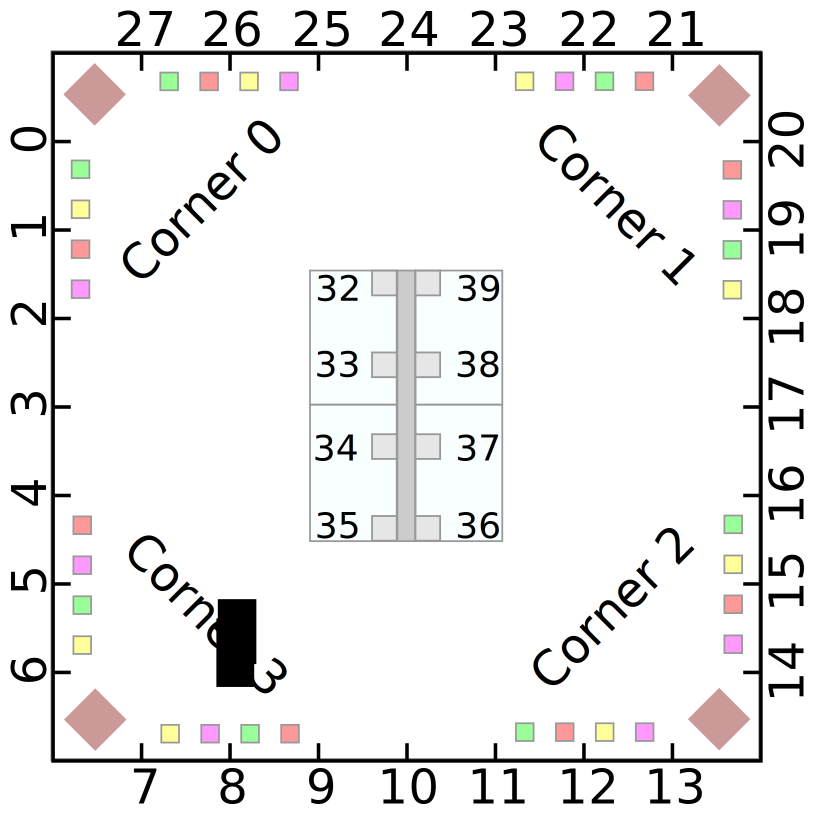
\includegraphics{./images/arena-markers.pdf}
    \caption{The positions of the four zones in the arena.
             The shaded area forms zone 1, and the other zones are rotationally symmetric to this.
             The numbers shown around the perimeter of this diagram are the numbers of the markers positioned on the wall.}
    \label{fig:arena-zones}
  \end{figure}

\item Each wall of the arena features seven $250mm$ libkoki markers.
      Figure~\ref{fig:arena-wall} shows the positioning of these markers, whilst figure~\ref{fig:arena-zones} shows the numbering of these markers.

  \begin{figure}
    \centering
    \includegraphics[width=\textwidth]{./images/sidewall.pdf}
    \caption{Seven $250mm$ wide markers are spaced evenly along each $8m$ arena wall.
             The markers are placed $50mm$ above the floor.}
    \label{fig:arena-wall}
  \end{figure}

\end{enumerate}

\subsection{Tokens}
\label{sub:Tokens}
\begin {enumerate}
\item Tokens are cubic corrugated cardboard boxes with side $110 \pm 10 mm$.
      \emph{Each team's kit contains four of these.}

\item Each token is associated with its own libkoki marker number.
      Each token is labelled with six identical $100mm$ libkoki markers -- one on each face.
\end {enumerate}

\subsection{Buckets}
\label{sub:buckets}
\begin{figure}
  \centering
  \includegraphics{./images/bucket-3d.pdf}
  \caption{Dimensions of the bucket.
 The height shown is the height from the bottom of the casters mounted on the base of the bucket to the top of the bucket's wall.}
  \label{fig:bucket-3d}
\end{figure}

\begin{enumerate}
\item Buckets are cuboid structures with the dimensions shown in figure~\ref{fig:bucket-3d}.
      These buckets are made from some commercially available storage boxes, bolted onto a $6mm$ thick MDF base.
      Casters are mounted on the underside of the buckets, allowing the bucket to be pushed or pulled around.
      \textit{The walls of the bucket are not flat.
      A guide on how to assemble a bucket, and where to obtain suitable parts can be found on the Student Robotics website.}

\item A $900mm$ long, $15mm$ diameter wooden dowel pole extends vertically from the centre of the bucket.
      Combined with the bucket barrier, this prevents buckets from entering the central area of the arena.
      To support this pole, a block of $45 \times 70mm$ pine lies across the centre of the bucket's base -- from long side to long side.
      The pole protrudes from the centre of this block, which has its $70mm$ face flat against the base.

\item Each bucket features two marker numbers: one which is used on the shorter sides of the bucket (a.k.a. ``the bucket ends''),
       and one that is used on the other vertical sides of the bucket.
      The markers on a given bucket will have the same offset (the difference between a markers number and the number of the first marker in the group),
       for example markers \#73 and \#77, both with offset 1, will be on the same bucket.
      These markers are $100mm$ in width, and are placed in the centre of the bucket faces that they occupy.

\end{enumerate}

\clearpage

\newpage
\input {awards}

\renewcommand{\labelenumi}{\rcn}

\section{Clarifications}
Requests for rule clarifications may be made on the Student Robotics forums, and this document will be updated if deemed necessary.  Requests received within one month of the competition are unlikely to be processed.

The following changes have been made to the rules since their initial release:

\begin{enumerate}
  \item 2014-11-10: Change rule 1.6 to refer to \emph{match officials} rather than a \emph{judge}.
  \item 2014-11-10: Change the gap between zones (including the barriers) from $300mm$ to $400mm$.
                    This ensures that a flag cannot be in more than one zone, even diagonally.
  \item 2014-11-10: Require that robots do not touch multiple flags at once.
  \item 2014-12-05: Remove invalid references to "slots" left over from SR2014.
  \item 2015-02-20: Clarify the size and position of the flag adornments.
\end{enumerate}

\newpage
\appendix
\appendixpage
\addappheadtotoc
\input {kit-return}
\input {safety-regs}

\end {document}
